\documentclass[conference]{IEEEtran}

\IEEEoverridecommandlockouts

\usepackage{cite}
\usepackage{amsmath,amssymb,amsfonts}
\usepackage{graphicx}
\usepackage{textcomp}
\usepackage{xcolor}
\usepackage{booktabs}
\usepackage{multirow}
\usepackage{array}
\usepackage{tabularx}
\usepackage{url}
\usepackage{hyperref}
\usepackage{float}
\usepackage{enumitem}
\usepackage{stfloats}

\hypersetup{
    colorlinks=true,
    linkcolor=blue,
    citecolor=blue,
    urlcolor=blue
}

\setlength{\columnsep}{0.24in}

\newcommand{\safeimage}[3]{
\begin{figure*}[t]
\centering
\IfFileExists{#1}{
    \includegraphics[width=#2\textwidth]{#1}
}{
    \fbox{\parbox{0.88\textwidth}{\centering Missing figure file: \texttt{#1}\\Upload this graph/image to Overleaf.}}
}
\caption{#3}
\end{figure*}
}

\begin{document}

\title{
Quality-Aware Low-Resource Pashto Neural Machine Translation:
Semantic Filtering, LoRA Adaptation, Multilingual Baselines,
and Pivot-Based Hindi Translation
}

\author{
\IEEEauthorblockN{Hrithik Sharma}
\IEEEauthorblockA{
Carnot Internship Research Project\\
Artificial Intelligence and Machine Learning\\
\href{https://github.com/Hrithikcrick/pashto-nmt-carnot-internship}{github.com/Hrithikcrick/pashto-nmt-carnot-internship}
}
}

\maketitle

\begin{abstract}
Low-resource neural machine translation is constrained not
only by corpus size but also by duplication, weak alignment,
domain mismatch, and unreliable evaluation. This paper
presents a quality-aware Pashto--English translation pipeline
using NLLB-200, semantic sentence-pair filtering, and LoRA
parameter-efficient adaptation, together with direct and
pivot-based Hindi extensions. Starting from 93,498 raw
Pashto--English sentence pairs, rule-based cleaning retained
90,978 pairs. Standardized evaluation was conducted on the
same 100 Pashto--English examples for the
pretrained NLLB baseline, original LoRA, semantic-filtered
LoRA, M2M100, and mBART-50. The pretrained NLLB model
obtained BLEU 19.63, chrF++ 35.48,
TER 75.68, and COMET 0.6818.
Original LoRA obtained BLEU 19.77,
chrF++ 36.31, TER
76.83, and COMET
0.6775. Semantic-filtered LoRA achieved
the highest BLEU and chrF++ values among the NLLB variants
at 20.38 and 36.61,
respectively, while its COMET score of
0.6819 remained approximately tied
with the pretrained baseline. The revised experimental
package additionally introduces informative pipeline and
metric visualizations, external multilingual baselines,
qualitative translation examples, paired bootstrap analysis,
automatic diagnostics, source-grouped leakage-controlled
splits, dataset checksums, experiment manifests, and
multi-seed configurations. The results support semantic
filtering as a useful data-selection strategy for LoRA
adaptation, but do not establish broad statistically
significant superiority over the strong multilingual baseline.
\end{abstract}

\begin{IEEEkeywords}
Low-resource machine translation, Pashto, NLLB, LoRA, PEFT, Hugging Face, semantic filtering, BLEU, chrF, pivot translation, Hindi translation, IndicTrans2.
\end{IEEEkeywords}

\section{Introduction}

Neural Machine Translation (NMT) has significantly improved translation quality for high-resource languages such as English, French, German, Spanish, Hindi, and Chinese. Large multilingual models can now translate between hundreds of languages with reasonable fluency. However, low-resource languages still face major limitations because they do not have sufficient high-quality parallel corpora. Pashto is one such language. Although Pashto has millions of speakers, the amount of publicly available, clean, and evaluation-ready parallel data is much smaller than what is available for high-resource language pairs.

The difficulty of Pashto translation is not only caused by limited dataset size. The quality of available data is equally important. Publicly available low-resource datasets often contain duplicated rows, very short sentence pairs, extremely long mismatched pairs, noisy web text, untranslated fragments, URL-heavy content, inconsistent script usage, and weak semantic alignment. If such data is used directly for training, the model may learn noisy mappings and produce incomplete, literal, or hallucinated translations.

This paper presents a structured Pashto NMT research pipeline that uses a pretrained multilingual translation model, performs dataset cleaning, evaluates baseline translation quality, prepares high-quality subsets, applies semantic similarity filtering, integrates manual error analysis, and then applies LoRA-based parameter-efficient fine-tuning. The baseline model used in this work is \texttt{facebook/nllb-200-distilled-600M}. The project focuses primarily on Pashto-to-English translation because English references are available for automatic evaluation. Direct Pashto-to-Hindi and pivot-based Pashto-to-English-to-Hindi translation are also included as extended translation directions.

The work is designed as a practical research pipeline rather than only a model training experiment. It includes dataset engineering, evaluation design, metric analysis, semantic filtering, error categorization, fine-tuning, Hindi comparison, and improvement planning. This is important because in low-resource NMT, model choice alone is not enough. Data quality, evaluation reliability, and error analysis strongly influence the final translation quality.

\section{Motivation}

Low-resource machine translation systems face several practical problems. A pretrained multilingual model may generate fluent output, but fluency does not always mean correctness. In Pashto translation, the model may omit important words, mistranslate named entities, change tense, produce overly literal English, or hallucinate content that is not present in the source sentence. These errors are especially harmful when translation is used for research, education, information access, or downstream multilingual applications.

A second motivation is the need for Hindi translation. Direct Pashto-to-Hindi translation is difficult because high-quality Pashto-Hindi parallel data is limited. A pivot-based strategy can be more practical: Pashto is first translated into English, and then English is translated into Hindi. If the Pashto-to-English stage improves, the downstream Hindi translation can also improve.

A third motivation is computational practicality. Full fine-tuning of large multilingual models is expensive. LoRA provides a practical solution by training only a small number of adapter parameters while keeping most pretrained model weights frozen. This makes fine-tuning possible under limited compute and storage constraints.

\section{Research Questions}

This work is guided by the following research questions:

\begin{itemize}
    \item How much noisy data can be removed from the raw Pashto-English dataset through rule-based cleaning?
    \item How strong is the pretrained NLLB model as a Pashto-to-English baseline?
    \item Can semantic similarity filtering improve the quality of the training subset?
    \item Can LoRA fine-tuning improve chrF over the baseline model?
    \item Does semantic-filtered LoRA perform better than original LoRA training?
    \item Why is manual error analysis necessary beyond BLEU and chrF?
    \item Is pivot-based Hindi translation more promising than direct Pashto-to-Hindi translation?
    \item What further steps are required to move toward deployment-level translation quality?
\end{itemize}

\section{Research Contributions}

The revised study makes the following contributions:

\begin{enumerate}
    \item A complete low-resource Pashto--English NMT
    pipeline based on NLLB-200 and LoRA.
    \item Rule-based cleaning of a 93,498-pair corpus,
    retaining 90,978 parallel sentence pairs.
    \item Semantic similarity filtering and filtered
    training subsets containing 8k, 4k, and 2k pairs.
    \item Standardized comparison of pretrained NLLB,
    original LoRA, and semantic-filtered LoRA on the
    same test instances.
    \item External zero-shot comparisons with M2M100
    and mBART-50 \cite{m2m100,mbart50}.
    \item Evaluation using BLEU, chrF++, TER, and
    COMET \cite{comet}.
    \item Paired bootstrap confidence intervals and
    significance analysis.
    \item Automatic diagnostics for number mismatch,
    output length, repetition, empty output, and exact
    reference matching.
    \item Informative research-pipeline and
    model-comparison figures.
    \item Qualitative baseline-versus-LoRA improvement
    and regression candidates.
    \item Fixed source-grouped splits with zero
    source-level and exact-pair leakage.
    \item Dataset hashes, environment records, training
    manifests, and reproducible experiment configurations.
    \item Controlled configurations for seeds 13, 42,
    and 2026.
    \item A successfully validated LoRA smoke-training
    and adapter-loading pipeline.
    \item Direct and pivot Hindi analysis, with
    IndicTrans2 retained only for the applicable
    English-to-Hindi pivot stage.
\end{enumerate}

\section{Related Work}

Multilingual NMT has become an important direction for low-resource languages because a single model can share representations across many languages. The No Language Left Behind (NLLB) model was developed to improve translation coverage for more than 200 languages, including many low-resource languages \cite{nllb}. NLLB is suitable for this project because it supports Pashto, English, and Hindi with explicit language codes.

LoRA, or Low-Rank Adaptation, is a parameter-efficient fine-tuning method that freezes the base model and introduces trainable low-rank matrices into selected layers \cite{lora}. This approach reduces trainable parameter count and makes adaptation practical under limited compute. In this project, LoRA is applied to selected attention projection modules of the NLLB model.

BLEU is a widely used metric for machine translation evaluation \cite{bleu}. It measures n-gram overlap between generated translations and references. However, BLEU can be harsh for morphologically rich and low-resource settings. chrF, based on character n-gram F-score, can better reflect partial lexical and morphological similarity \cite{chrf}. Therefore, this project reports both BLEU and chrF.

\section{System Overview}

The complete research pipeline consists of the following stages:

\begin{enumerate}
    \item Collection of Pashto-English parallel data.
    \item Conversion of raw data into structured CSV format.
    \item Dataset cleaning and noise removal.
    \item Train-validation-test split creation.
    \item Baseline translation using NLLB.
    \item Evaluation using BLEU, chrF, and inference time.
    \item High-quality 10k subset construction.
    \item Semantic similarity filtering.
    \item Gold test candidate preparation.
    \item LoRA-based fine-tuning.
    \item Semantic-filtered LoRA fine-tuning.
    \item Baseline versus fine-tuned checkpoint comparison.
    \item Direct Hindi versus pivot Hindi comparison.
    \item IndicTrans2 exploration for improved Hindi generation.
    \item Improved LoRA experiment planning.
\end{enumerate}

\section{Dataset Preparation}

\subsection{Raw Dataset}

The project uses Pashto-English parallel data converted into CSV format. The raw dataset contained 93,498 sentence pairs. Each row contains a Pashto source sentence and an English target sentence.

\subsection{Cleaning Strategy}

The cleaning pipeline removes duplicate, noisy, and weakly useful rows. The cleaning rules include:

\begin{itemize}
    \item Removing empty rows.
    \item Removing duplicate sentence pairs.
    \item Removing URL-heavy and HTML-contaminated text.
    \item Removing very short sentence pairs.
    \item Removing extremely long sentence pairs.
    \item Removing rows with extreme source-target length ratio.
    \item Checking script consistency for Pashto and English text.
\end{itemize}

\subsection{Dataset Cleaning Summary}

\begin{table}[H]
\centering
\caption{Dataset cleaning summary.}
\begin{tabular}{lr}
\toprule
\textbf{Stage} & \textbf{Rows} \\
\midrule
Raw sentence pairs & 93,498 \\
After duplicate removal & 93,418 \\
Final clean sentence pairs & 90,978 \\
Removed noisy rows & 2,440 \\
\bottomrule
\end{tabular}
\end{table}

\section{Dataset Split}

The cleaned dataset was divided into training, validation, and test splits. The training split contains 72,782 rows, while validation and test splits contain 9,098 rows each.

\begin{table}[H]
\centering
\caption{Train-validation-test split.}
\begin{tabular}{lr}
\toprule
\textbf{Split} & \textbf{Rows} \\
\midrule
Training & 72,782 \\
Validation & 9,098 \\
Test & 9,098 \\
\bottomrule
\end{tabular}
\end{table}

\section{Baseline Translation Model}

\subsection{Model Selection}

The baseline model used in this project is:

\begin{center}
\texttt{facebook/nllb-200-distilled-600M}
\end{center}

The model was selected because it supports multilingual translation across many languages, including Pashto, English, and Hindi. It provides a strong starting point for low-resource translation without training a model from scratch.

\subsection{Language Codes}

\begin{table}[H]
\centering
\caption{NLLB language codes used in this project.}
\begin{tabular}{ll}
\toprule
\textbf{Language} & \textbf{NLLB Code} \\
\midrule
Pashto & \texttt{pbt\_Arab} \\
English & \texttt{eng\_Latn} \\
Hindi & \texttt{hin\_Deva} \\
\bottomrule
\end{tabular}
\end{table}

\subsection{Translation Directions}

The system supports:

\begin{itemize}
    \item Pashto-to-English translation.
    \item Direct Pashto-to-Hindi translation.
    \item Pivot-based Pashto-to-English-to-Hindi translation.
\end{itemize}

\section{Baseline Evaluation}

\subsection{Standardized Automatic Metrics}

The earlier preliminary baseline values were replaced by a
standardized evaluation computed from the same prediction
and reference files used for all NLLB-based systems.

\begin{table}[H]
\centering
\caption{Standardized NLLB baseline evaluation.}
\label{tab:standardized-baseline}
\begin{tabular}{lr}
\toprule
\textbf{Metric} & \textbf{Score} \\
\midrule
BLEU & 19.63 \\
chrF++ & 35.48 \\
TER & 75.68 \\
COMET & 0.6818 \\
\bottomrule
\end{tabular}
\end{table}

BLEU and chrF++ are higher-is-better metrics, whereas TER
is lower-is-better. COMET provides a complementary neural
evaluation signal. All reported systems use the same
100-sentence evaluation set.

\subsection{Inference-Time Analysis}

The previously measured CPU inference-time comparison is
retained as an engineering observation. It is not treated as
a translation-quality metric.

\begin{table}[H]
\centering
\caption{Average CPU inference time.}
\begin{tabular}{lr}
\toprule
\textbf{Translation Direction} &
\textbf{Time per Sentence} \\
\midrule
Pashto-to-English & 4.46 sec \\
Pashto-to-Hindi Direct & 5.11 sec \\
Pashto-to-English-to-Hindi Pivot & 4.76 sec \\
\bottomrule
\end{tabular}
\end{table}

\section{Dataset Quality Integration}

\subsection{High-Quality Subset}

A high-quality 10,000-pair subset was prepared from the cleaned dataset. This subset was selected for fine-tuning because training on a smaller but cleaner dataset can be more effective than training on a larger noisy dataset.

\subsection{Gold Test Candidate Set}

A 100-sample gold test candidate set was prepared for controlled evaluation. This test set allows direct comparison between the baseline and fine-tuned models.

\subsection{Final Dataset Resources}

\begin{table}[H]
\centering
\caption{Final dataset resources.}
\begin{tabular}{lrl}
\toprule
\textbf{File} & \textbf{Rows} & \textbf{Purpose} \\
\midrule
\texttt{cleaned\_90k.csv} & 90,978 & Clean corpus \\
\texttt{train\_high\_quality\_10k.csv} & 10,000 & Fine-tuning data \\
\texttt{gold\_test\_candidates\_100.csv} & 100 & Evaluation candidates \\
\bottomrule
\end{tabular}
\end{table}

\section{Semantic Similarity Filtering}

Rule-based cleaning removes obvious noisy pairs, but it cannot always detect weak semantic alignment. Therefore, an additional semantic similarity filtering stage was added. The goal is to score Pashto-English sentence pairs using multilingual sentence embeddings and retain the most semantically aligned examples for future fine-tuning.

The semantic filtering process follows these steps:

\begin{enumerate}
    \item Encode Pashto source sentences using a multilingual sentence embedding model.
    \item Encode English target sentences using the same embedding model.
    \item Compute cosine similarity between source and target embeddings.
    \item Sort sentence pairs by semantic similarity score.
    \item Retain the best aligned sentence pairs for fine-tuning.
\end{enumerate}

\begin{equation}
\text{sim}(x,y)=\frac{x \cdot y}{\|x\|\|y\|}
\end{equation}

A multilingual sentence-transformer model was used for this stage. The filtering stage generated pair-level semantic similarity scores, filtered training subsets, top high-similarity examples, and summary statistics.

\begin{table}[H]
\centering
\caption{Semantic filtering outputs.}
\footnotesize
\begin{tabular}{p{0.44\linewidth}p{0.43\linewidth}}
\toprule
\textbf{Output} & \textbf{Purpose} \\
\midrule
Semantic similarity scores & Pair-level similarity scoring \\
Filtered 8000-pair dataset & Main filtered training subset \\
Top 2000 clean subset & Cleaner small training subset \\
Top 4000 clean subset & Cleaner medium training subset \\
Top examples preview & Manual inspection of best pairs \\
\bottomrule
\end{tabular}
\end{table}

\subsection{Semantic Filtering Interpretation}

The semantic filtering step improves the data-quality pipeline by ranking sentence pairs according to cross-lingual similarity. Higher similarity values indicate better alignment between the Pashto source sentence and the English reference sentence. Lower similarity values may indicate noisy, mismatched, incomplete, or weakly translated sentence pairs.

This step is important in low-resource NMT because a smaller clean dataset can sometimes produce better fine-tuning results than a larger noisy dataset. The filtered 8000-pair dataset and the top 2000/top 4000 clean subsets were therefore prepared for improved LoRA experiments.

\section{Qualitative Error Analysis Framework}

Automatic metrics cannot fully explain omissions,
hallucinations, named-entity errors, number errors,
tense changes, literal translation, or poor fluency.
The project therefore defines a qualitative analysis
framework covering:

\begin{itemize}
    \item missing or omitted information;
    \item incorrect or changed meaning;
    \item incomplete translation;
    \item named-entity and number errors;
    \item tense and grammatical mismatch;
    \item literal or unnatural translation;
    \item hallucinated content;
    \item untranslated text and repetition.
\end{itemize}

A structured evaluation template was prepared for future
bilingual annotation. However, a formal human evaluation
has not yet been completed. The examples reported in this
paper are automatically selected comparison candidates and
must not be interpreted as human preference judgments.

\section{LoRA Fine-Tuning}

\subsection{Motivation}

Full fine-tuning of NLLB is computationally expensive. LoRA is selected because it trains a small number of adapter parameters while freezing most of the base model. This reduces memory requirements and makes fine-tuning more practical.

\subsection{Original LoRA Configuration}

\begin{table}[H]
\centering
\caption{Original LoRA fine-tuning configuration.}
\footnotesize
\begin{tabular}{p{0.34\linewidth}p{0.52\linewidth}}
\toprule
\textbf{Component} & \textbf{Configuration} \\
\midrule
Base model & NLLB 600M \\
Source language & \texttt{pbt\_Arab} \\
Target language & \texttt{eng\_Latn} \\
Fine-tuning method & LoRA \\
LoRA rank & 8 \\
LoRA alpha & 16 \\
LoRA dropout & 0.05 \\
Target modules & \texttt{q\_proj}, \texttt{v\_proj} \\
Training data & High-quality 10k subset \\
Evaluation data & 100 gold candidates \\
\bottomrule
\end{tabular}
\end{table}

\subsection{Semantic-Filtered LoRA Configuration}

A semantic-filtered LoRA experiment was added after semantic similarity filtering. The semantic-filtered LoRA model was trained using the filtered Pashto-English subset and evaluated on the same gold test candidate set.

\begin{table}[H]
\centering
\caption{Semantic-filtered LoRA experiment.}
\footnotesize
\begin{tabular}{p{0.34\linewidth}p{0.52\linewidth}}
\toprule
\textbf{Component} & \textbf{Configuration} \\
\midrule
Base model & NLLB 600M \\
Fine-tuning method & LoRA \\
Training data & Semantic-filtered 8000-pair subset \\
Evaluation data & 100 gold test candidates \\
Output file & Semantic LoRA prediction CSV \\
Score file & Semantic LoRA BLEU/chrF score CSV \\
\bottomrule
\end{tabular}
\end{table}

The long repository filenames were kept in the GitHub project for reproducibility, but shortened names are used in this paper to avoid layout overflow in IEEE two-column format.

\section{Fine-Tuning Results}

All NLLB-based systems were re-evaluated using the same
source sentences, English references, decoding outputs, and
metric implementations.

\begin{table}[H]
\centering
\caption{Standardized NLLB and LoRA results.}
\label{tab:nllb-lora-results}
\small
\begin{tabular}{lrrrr}
\toprule
\textbf{System} &
\textbf{BLEU} &
\textbf{chrF++} &
\textbf{TER} &
\textbf{COMET} \\
\midrule
Baseline NLLB &
19.63 &
35.48 &
75.68 &
0.6818 \\
Original LoRA &
19.77 &
36.31 &
76.83 &
0.6775 \\
Semantic LoRA &
20.38 &
36.61 &
76.45 &
0.6819 \\
\bottomrule
\end{tabular}
\end{table}

Semantic-filtered LoRA achieved the highest BLEU and
chrF++ point estimates among the NLLB variants. Relative
to the pretrained baseline, it increased corpus BLEU by
+0.75 and chrF++
by +1.12.
However, COMET changed by only
+0.000082, which is
effectively a tie. Its TER was also higher than the baseline.

Original LoRA improved chrF++ but produced a slightly lower
COMET score and a higher TER. The results therefore indicate
modest and metric-dependent improvement rather than uniform
superiority across all evaluation measures.

\section{Improved LoRA Experiments}

To improve translation quality beyond the initial LoRA results, additional experiments were designed using cleaner semantic-filtered data and stronger adapter settings.

\subsection{Improved Data Selection}

Two cleaner subsets were created from semantic similarity scores:

\begin{itemize}
    \item \texttt{train\_semantic\_top2000\_clean.csv}
    \item \texttt{train\_semantic\_top4000\_clean.csv}
\end{itemize}

These subsets additionally apply sentence length and length-ratio filtering. The motivation is that smaller but cleaner data may outperform larger noisy data in low-resource settings.

\subsection{Strong LoRA and Strong-v2 LoRA}

A heavier LoRA setting was tested using more trainable modules. However, local CPU/RAM constraints made the heaviest setup difficult to run. Therefore, a safer strong-v2 configuration was prepared using attention projection modules only.

\begin{table}[H]
\centering
\caption{Strong-v2 LoRA improvement setup.}
\footnotesize
\begin{tabular}{p{0.34\linewidth}p{0.52\linewidth}}
\toprule
\textbf{Component} & \textbf{Configuration} \\
\midrule
LoRA rank & 12 \\
LoRA alpha & 24 \\
Target modules & \texttt{q\_proj}, \texttt{k\_proj}, \texttt{v\_proj}, \texttt{out\_proj} \\
Dropout & 0.08 \\
Training data & Semantic top-clean subset \\
Goal & Improve chrF while avoiding CPU/RAM failure \\
\bottomrule
\end{tabular}
\end{table}

\subsection{Improved Experiment Interpretation}

The improved LoRA experiment tests whether stronger adapters and cleaner semantic-filtered data can improve translation quality beyond the original LoRA setup. A larger adapter can potentially learn better task-specific changes, but it also increases memory and compute requirements.

The strong-v2 configuration is therefore a practical compromise. It is stronger than the initial LoRA setup because it uses more attention projection modules, but it avoids the heavier feed-forward modules that caused local CPU/RAM failure. This makes it suitable for continued experimentation under limited hardware constraints.

\section{Direct Hindi and Pivot Hindi Translation}

The project explores Hindi translation through two approaches. The first approach is direct Pashto-to-Hindi translation using NLLB. The second approach is pivot translation, where Pashto is first translated into English and then English is translated into Hindi.

The pivot approach is promising because Pashto-to-English can be evaluated more reliably using English references. If the Pashto-to-English model improves, the downstream English-to-Hindi output can also improve.

\subsection{Direct-vs-Pivot Hindi Comparison}

A direct-vs-pivot Hindi comparison file was generated using the gold test candidates. Each sample contains the Pashto source, pivot English translation, direct Hindi output, pivot Hindi output, and manual review columns.

\begin{table}[H]
\centering
\caption{Hindi comparison outputs.}
\footnotesize
\begin{tabular}{p{0.34\linewidth}p{0.52\linewidth}}
\toprule
\textbf{Column} & \textbf{Purpose} \\
\midrule
Pashto source & Original input sentence \\
Pivot English & Intermediate English translation \\
Direct Hindi & Direct Pashto-to-Hindi output \\
Pivot Hindi & Pashto-to-English-to-Hindi output \\
Manual better method & Human comparison field \\
Manual comment & Error and quality notes \\
\bottomrule
\end{tabular}
\end{table}

This comparison is necessary because Hindi output cannot be judged reliably using BLEU or chrF without gold Hindi references. Manual review is therefore required to decide whether direct or pivot translation is better.

\section{IndicTrans2 Applicability and Status}

IndicTrans2 was considered for the English-to-Hindi stage
of the pivot translation pipeline:

\begin{center}
Pashto $\rightarrow$ English using NLLB/LoRA
$\rightarrow$ Hindi using IndicTrans2.
\end{center}

IndicTrans2 is not used as a direct Pashto-to-English
baseline in this study. Native Windows installation of the
official processing toolkit was not completed because its
Cython extension required an unavailable compiler toolchain.
The quantitative Pashto-to-English architecture comparison
was therefore conducted using NLLB, M2M100, and mBART-50.

Until IndicTrans2 outputs are generated in a supported
Linux or Colab environment, it is reported only as an
applicable future English-to-Hindi pivot experiment.
No IndicTrans2 quality result is claimed in this paper.

\section{Ablation Study}

A complete ablation study is needed to understand how data size, semantic filtering, and LoRA settings affect translation performance.

\begin{table}[H]
\centering
\caption{Ablation study design.}
\footnotesize
\begin{tabular}{p{0.11\linewidth}p{0.25\linewidth}p{0.22\linewidth}p{0.27\linewidth}}
\toprule
\textbf{ID} & \textbf{Model} & \textbf{Data} & \textbf{Purpose} \\
\midrule
E0 & NLLB & None & Baseline \\
E1 & NLLB+LoRA & 100 pairs & Pipeline test \\
E2 & NLLB+LoRA & 500 pairs & Small training \\
E3 & NLLB+LoRA & 1k pairs & Scaling test \\
E4 & NLLB+LoRA & 3k pairs & Medium training \\
E5 & NLLB+LoRA & 10k pairs & Main run \\
E6 & NLLB+LoRA & Semantic 8k & Filtering test \\
E7 & Strong-v2 LoRA & Top semantic 2k & Adapter test \\
E8 & Strong-v2 LoRA & Top semantic 4k & Larger clean-data test \\
\bottomrule
\end{tabular}
\end{table}

\section{Reproducibility}

The repository contains code for dataset processing, semantic filtering, fine-tuning, evaluation, checkpoint comparison, Hindi comparison, and report generation. The important files include:

\begin{itemize}
    \item \texttt{src/finetune\_nllb\_lora.py}
    \item \texttt{src/finetune\_nllb\_lora\_strong\_v2.py}
    \item \texttt{src/week5\_semantic\_filter.py}
    \item \texttt{src/evaluate\_week4\_model.py}
    \item \texttt{src/evaluate\_improved\_generation.py}
    \item \texttt{src/compare\_remaining\_checkpoints.py}
    \item \texttt{src/remaining\_direct\_vs\_pivot\_hindi.py}
    \item \texttt{data/train\_high\_quality\_10k.csv}
    \item \texttt{data/train\_semantic\_filtered\_8000.csv}
    \item \texttt{data/gold\_test\_candidates\_100.csv}
\end{itemize}

Large model checkpoints are not stored in the repository because they are too large for normal GitHub tracking. Instead, scripts, evaluation outputs, graphs, and reports are pushed to maintain reproducibility.

\section{Limitations}

The present study has the following limitations:

\begin{itemize}
    \item The standardized evaluation currently contains
    100 shared Pashto--English examples.
    \item Full three-seed training is not yet complete;
    seed configurations have been prepared but must still
    be executed.
    \item M2M100 and mBART-50 are evaluated zero-shot and
    have not yet received equal-budget LoRA adaptation.
    \item The qualitative examples are automatically
    selected and have not been validated by multiple
    bilingual annotators.
    \item BLEU, chrF++, TER, and COMET provide
    complementary but imperfect quality estimates.
    \item Hindi evaluation lacks a gold Hindi reference set.
    \item IndicTrans2 inference was not completed in the
    native Windows environment.
    \item CPU-only training limits the number of model,
    data-size, seed, and hyperparameter experiments.
    \item The current results do not establish
    state-of-the-art performance.
\end{itemize}

\section{Extended Evaluation and Instructor-Requested Improvements}

\subsection{Informative Research Pipeline}

The original screenshot-style summary figures were replaced
by an informative end-to-end research diagram connecting
corpus preparation, leakage control, semantic filtering,
LoRA adaptation, external baselines, automatic metrics,
qualitative analysis, and Hindi translation.

\begin{figure*}[t]
\centering
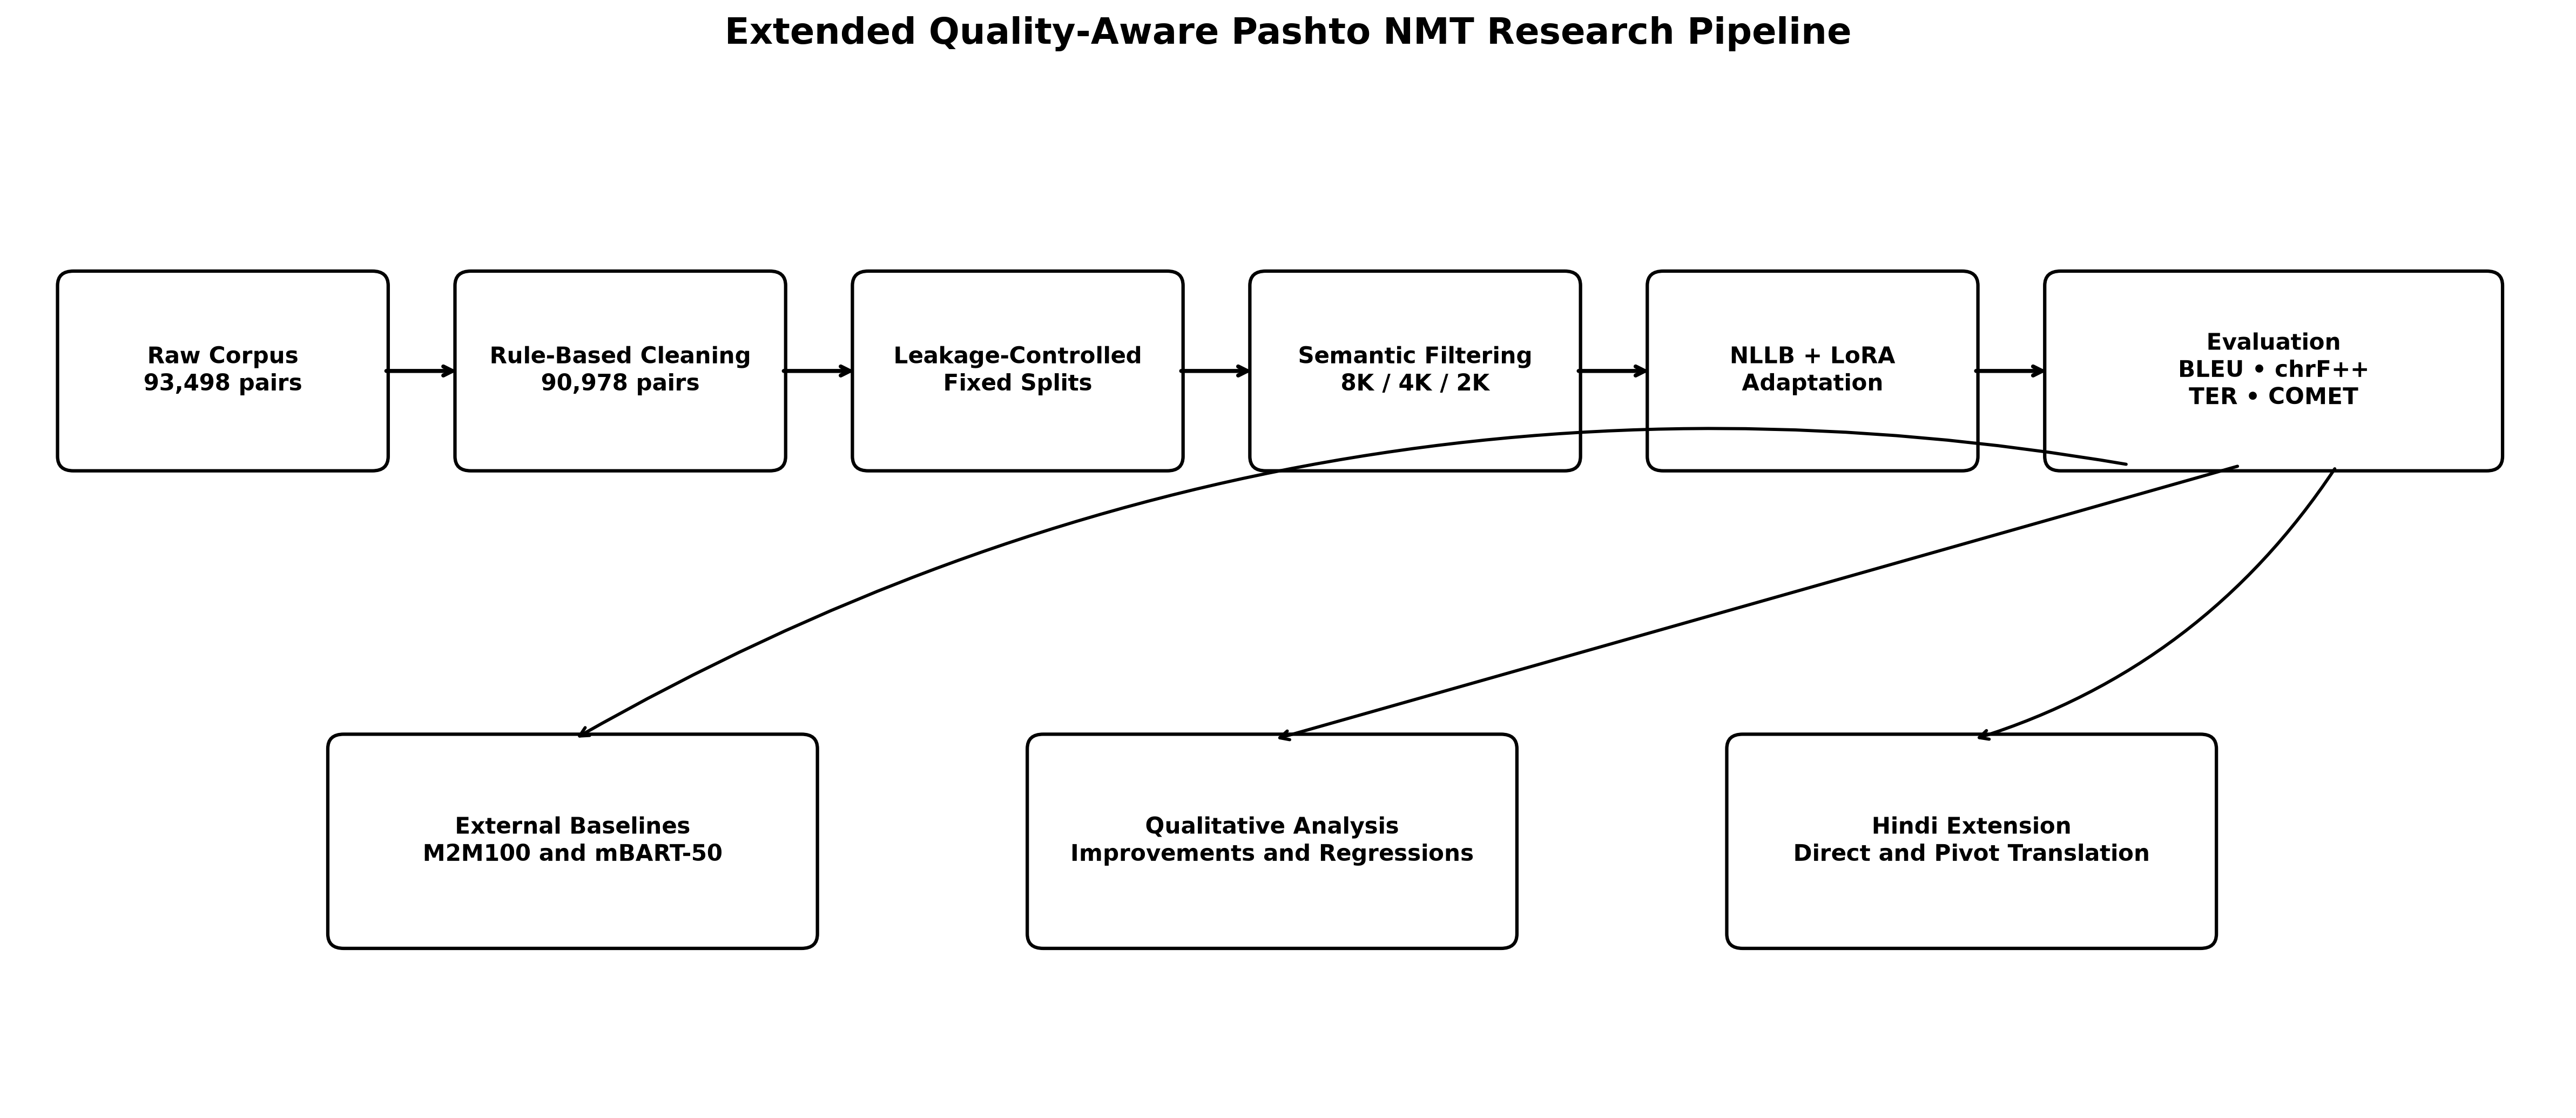
\includegraphics[
    width=0.98\textwidth
]{figures/instructor_extended_pipeline.png}
\caption{Extended quality-aware Pashto NMT research
pipeline.}
\label{fig:extended-pipeline}
\end{figure*}

\subsection{Multilingual Architecture Comparison}

To place NLLB in a broader multilingual context, M2M100
and mBART-50 were evaluated zero-shot on the same
Pashto--English instances \cite{m2m100,mbart50}.

\begin{table*}[t]
\centering
\caption{Standardized Pashto--English evaluation across NLLB, LoRA, and external multilingual baselines.}
\label{tab:extended-model-comparison}
\small
\begin{tabular}{lrrrrrl}
\toprule
\textbf{Model} & \textbf{BLEU} & \textbf{chrF++} & \textbf{TER} & \textbf{COMET} & \textbf{Samples} & \textbf{Setting} \\
\midrule
Baseline NLLB & 19.63 & 35.48 & 75.68 & 0.6818 & 100 & NLLB baseline or LoRA adaptation \\
Original LoRA & 19.77 & 36.31 & 76.83 & 0.6775 & 100 & NLLB baseline or LoRA adaptation \\
Semantic LoRA & 20.38 & 36.61 & 76.45 & 0.6819 & 100 & NLLB baseline or LoRA adaptation \\
M2M100 418M & 14.62 & 30.59 & 85.42 & 0.6169 & 100 & External zero-shot baseline \\
mBART-50 & 22.65 & 38.08 & 75.77 & 0.6932 & 100 & External zero-shot baseline \\
\bottomrule
\end{tabular}
\vspace{2pt}\parbox{0.95\textwidth}{\footnotesize TER is lower-is-better. M2M100 and mBART-50 are external zero-shot baselines and were not fine-tuned on the project corpus.}
\end{table*}

\begin{figure*}[t]
\centering
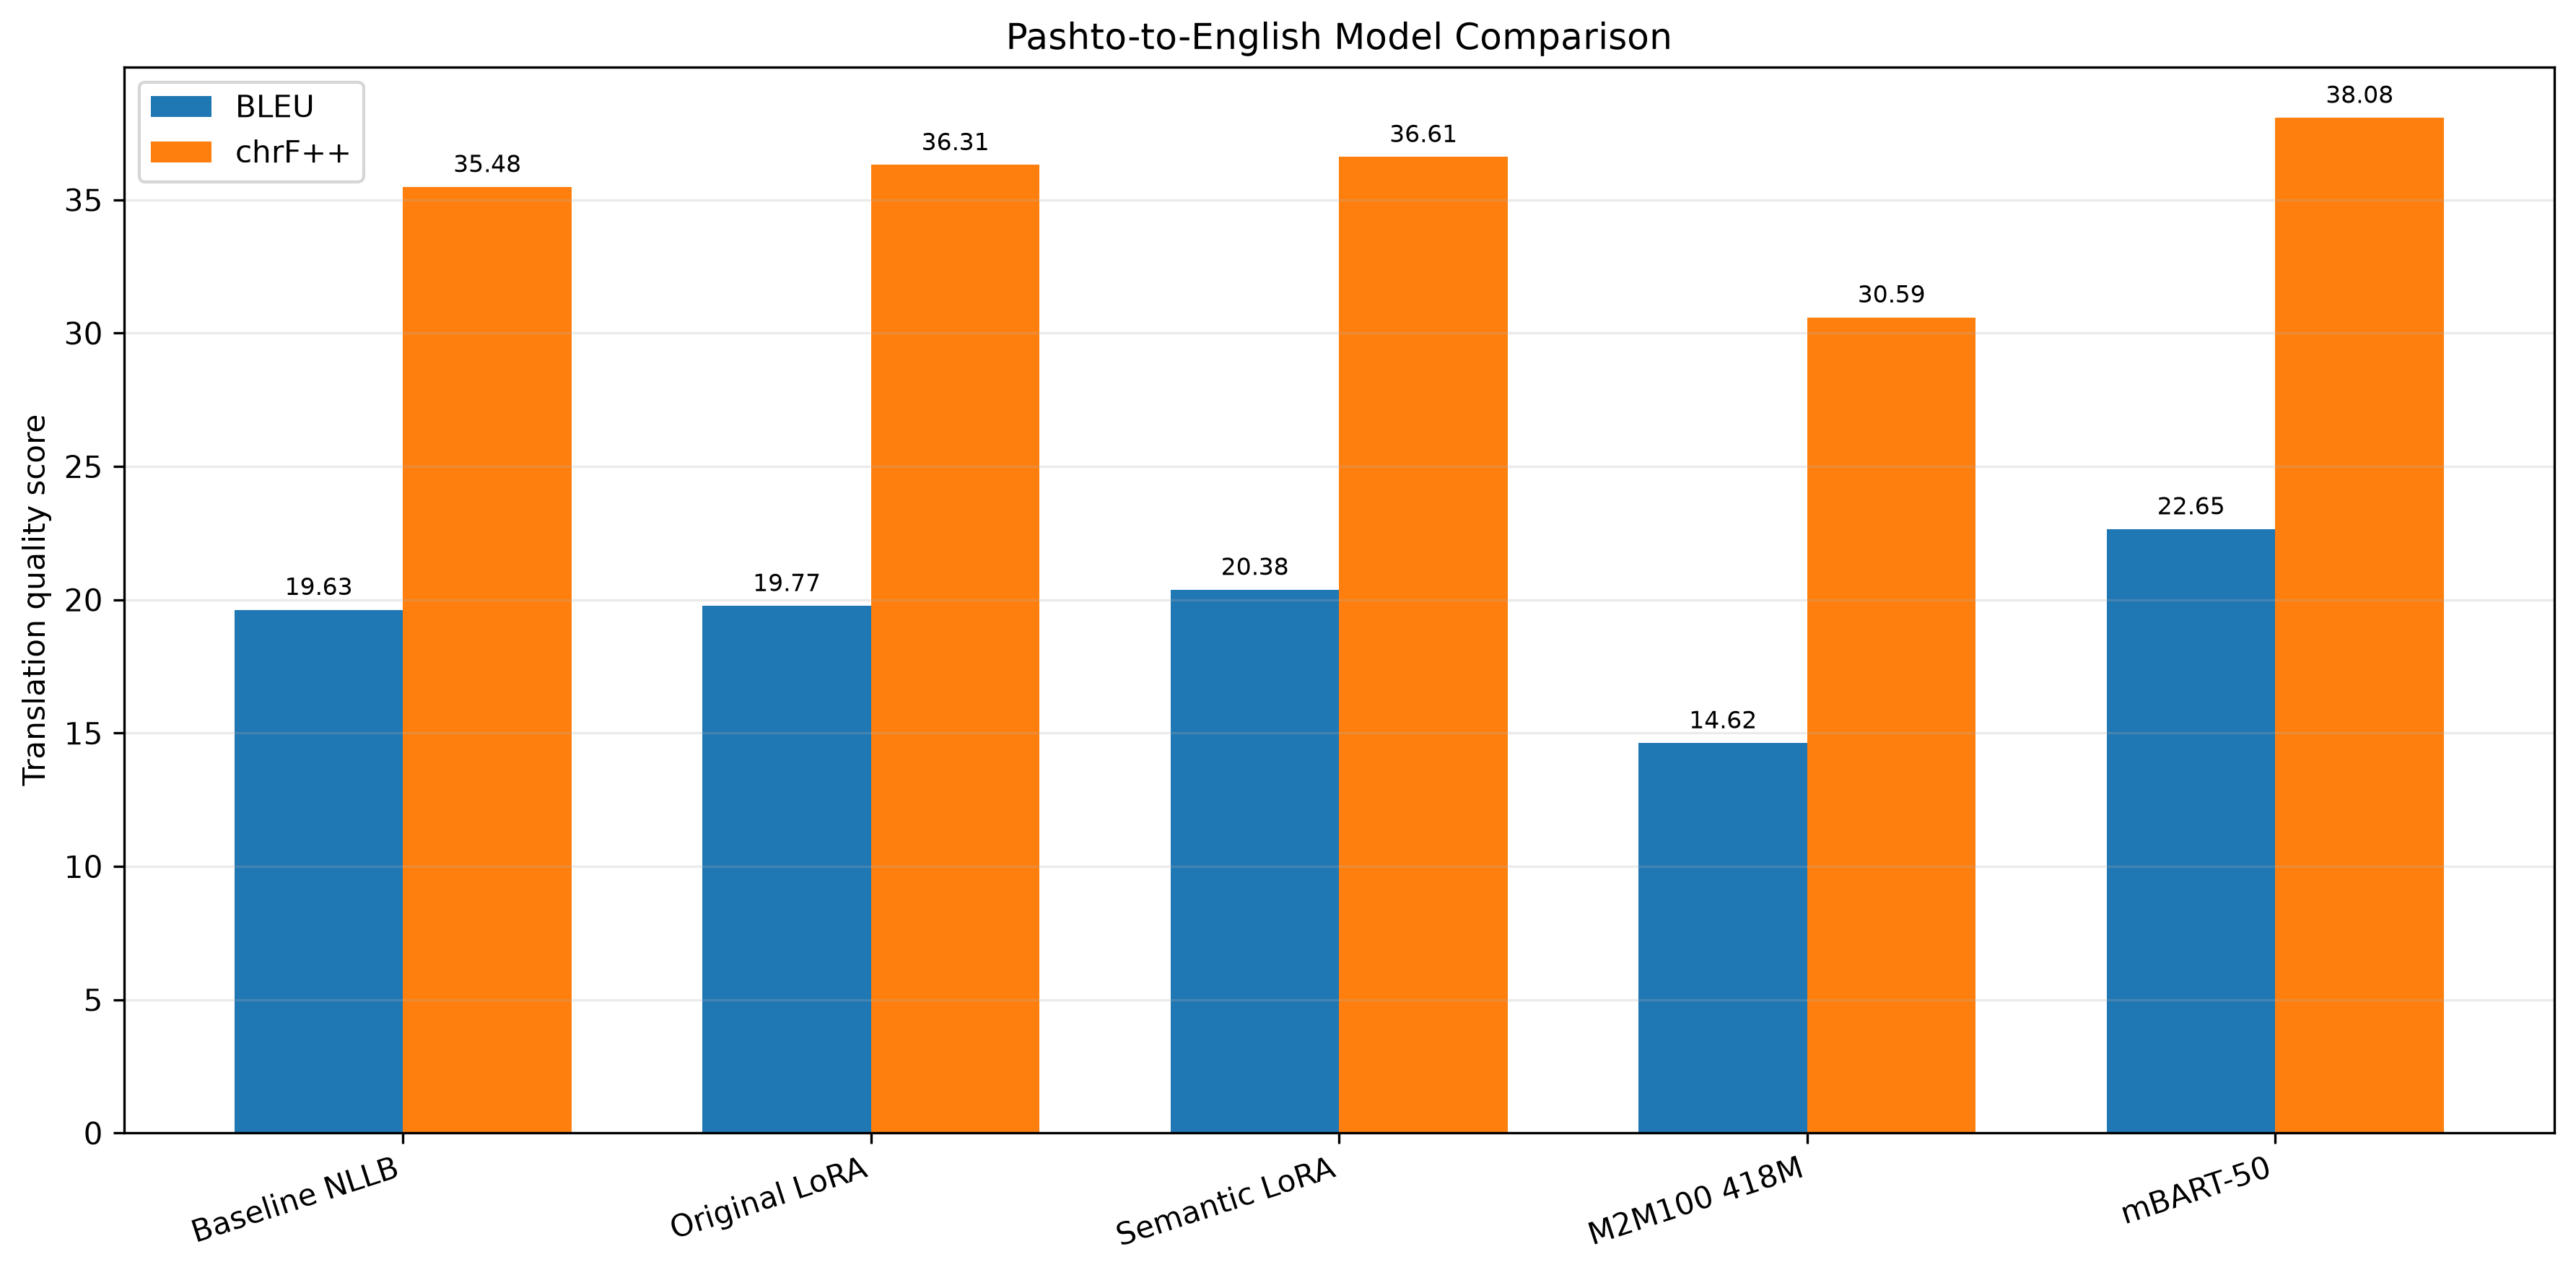
\includegraphics[
    width=0.92\textwidth
]{figures/instructor_model_quality_comparison.png}
\caption{BLEU and chrF++ comparison across the evaluated
NLLB, LoRA, M2M100, and mBART-50 systems.}
\label{fig:quality-comparison}
\end{figure*}

\begin{figure}[t]
\centering
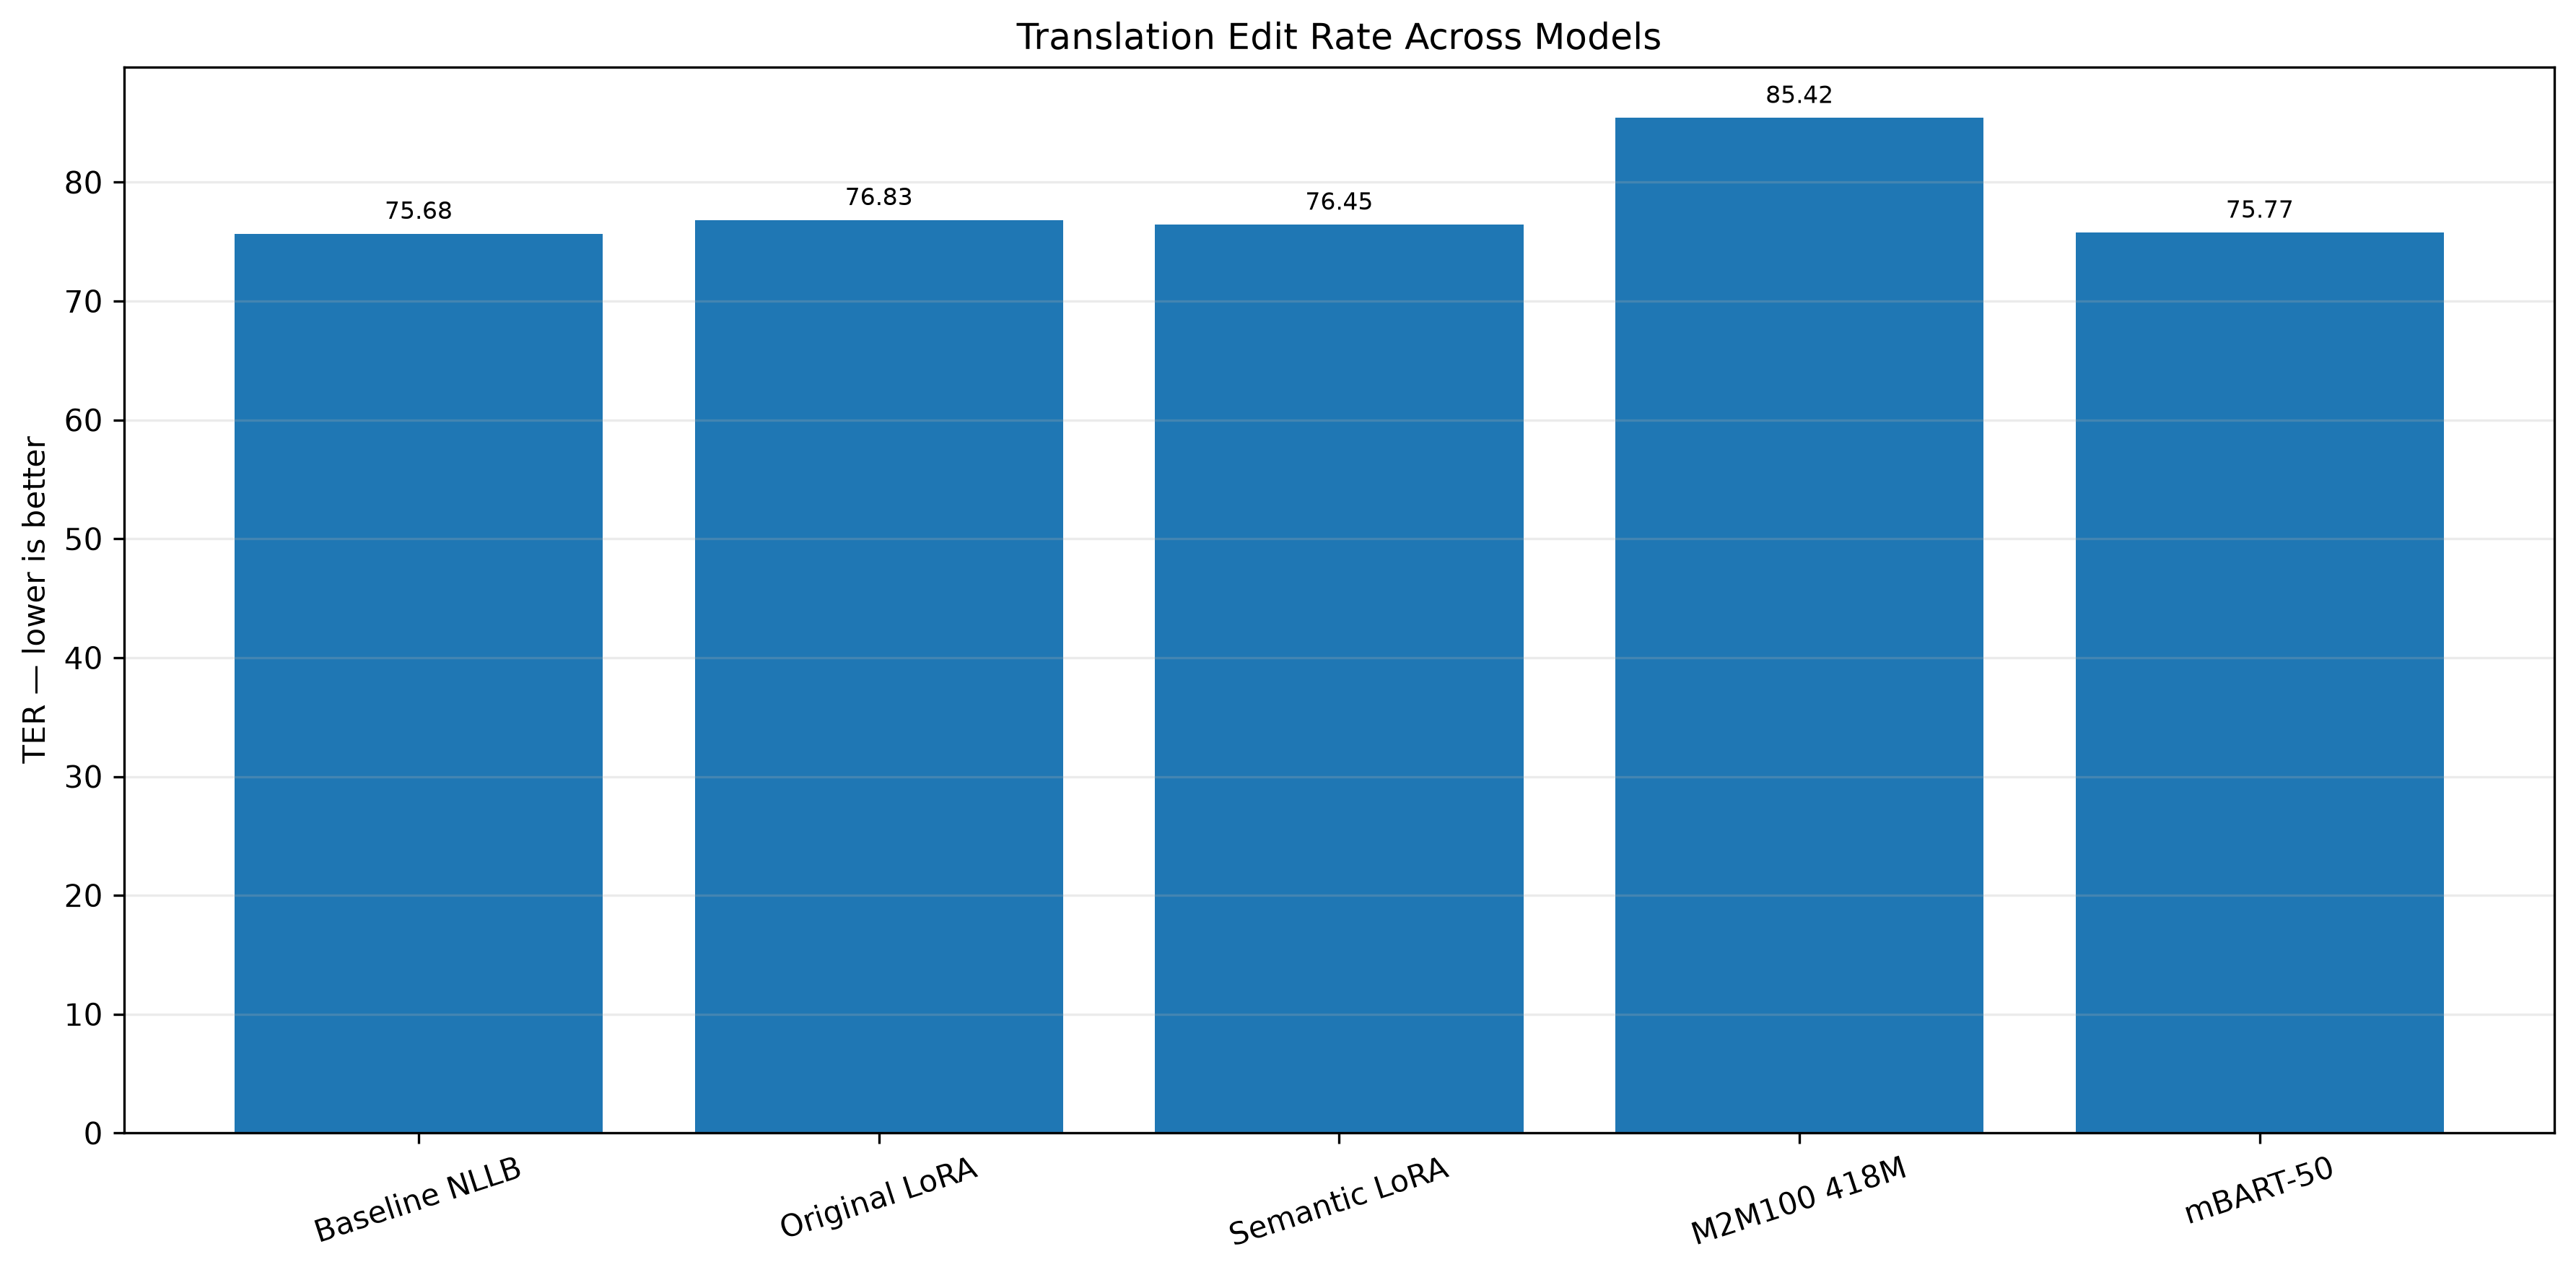
\includegraphics[
    width=\columnwidth
]{figures/instructor_model_ter_comparison.png}
\caption{Translation Edit Rate comparison. Lower values
are better.}
\label{fig:ter-comparison}
\end{figure}

\IfFileExists{
    figures/instructor_model_comet_comparison.png
}{
\begin{figure}[t]
\centering
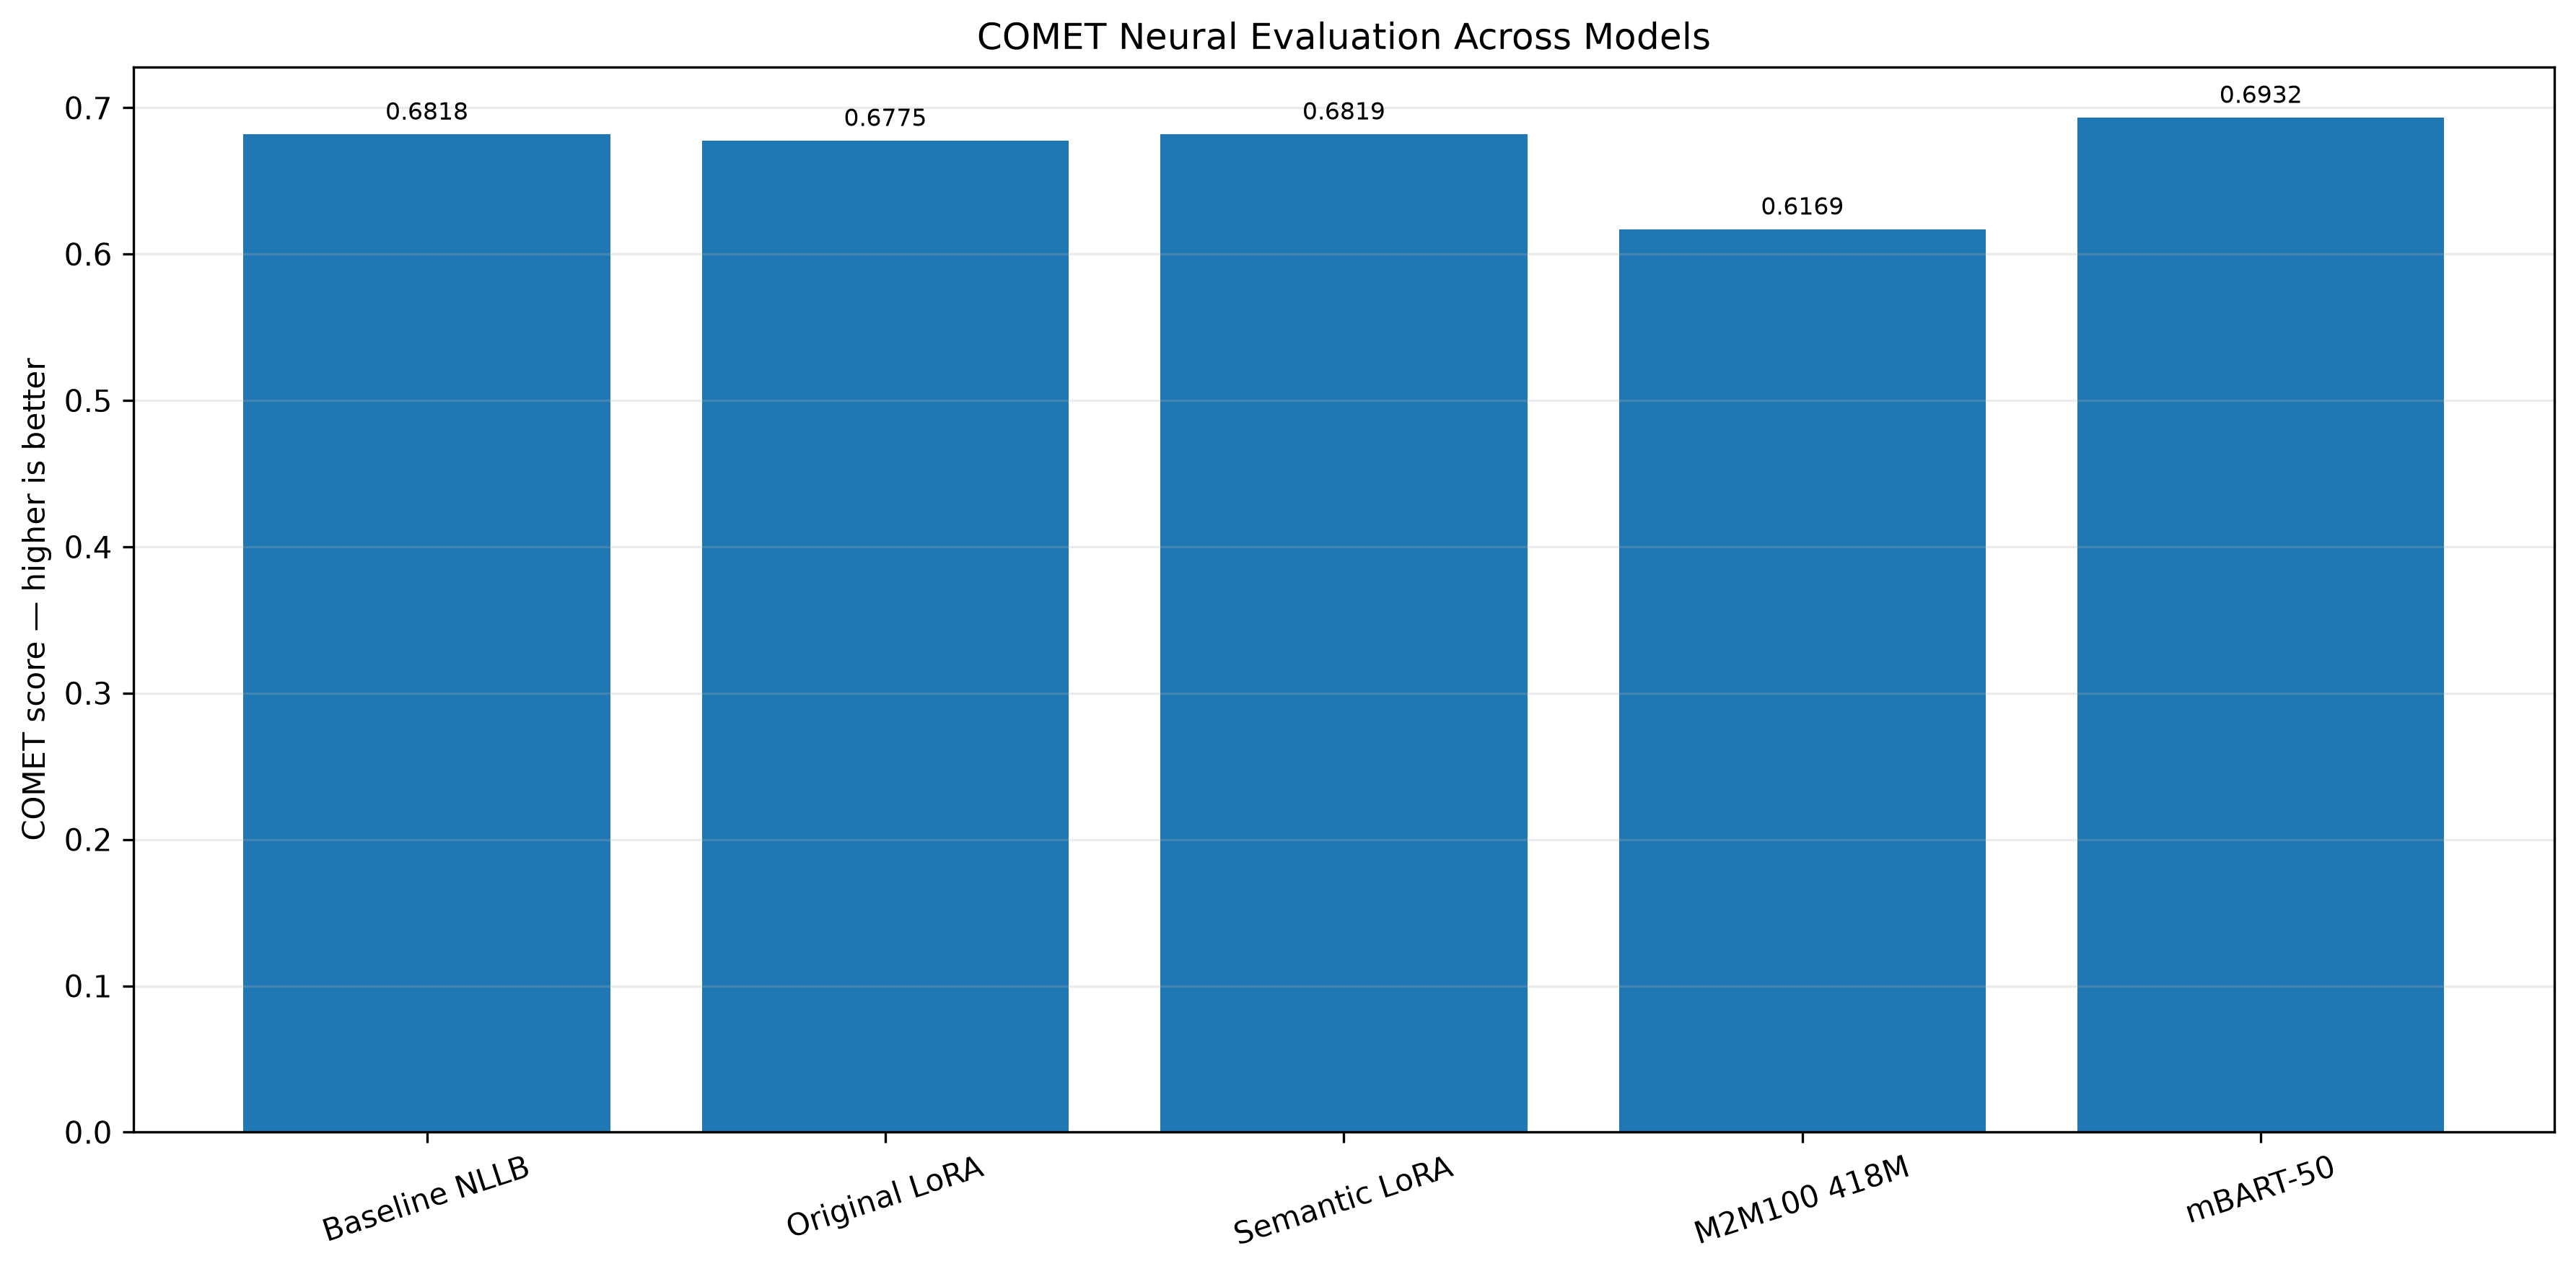
\includegraphics[
    width=\columnwidth
]{figures/instructor_model_comet_comparison.png}
\caption{COMET neural evaluation for systems with
completed COMET scores.}
\label{fig:comet-comparison}
\end{figure}
}{}

\subsection{Qualitative Translation Examples}

The instructor-requested qualitative examples compare the
English reference, pretrained NLLB output, original LoRA
output, and semantic-filtered LoRA output. Improvement and
regression candidates were selected using sentence-level
chrF++ differences. They illustrate model behaviour but do
not replace bilingual human evaluation.

\begin{table*}[t]
\centering
\caption{Qualitative comparison of baseline NLLB, original LoRA, and semantic-filtered LoRA outputs.}
\label{tab:qualitative-comparison}
\footnotesize
\begin{tabularx}{\textwidth}{p{0.16\textwidth}X}
\toprule
\multicolumn{2}{l}{\textbf{Example 1: Improvement candidate}} \\
Pashto source & په مادي توګه د فرعي لیستونو جوړولو لپاره برخه. \\
Reference & Segment manually to create sub-lists. \\
NLLB baseline & Physically part to form sub-lists. \\
Original LoRA & Physically part to create sub-lists. \\
Semantic LoRA & Physically part to create sub-lists. \\
chrF++ change & +24.31 (Semantic LoRA minus baseline) \\
\midrule
\multicolumn{2}{l}{\textbf{Example 2: Improvement candidate}} \\
Pashto source & د بحث سره یوځای غواړئ؟ \\
Reference & Want to join the discussion? \\
NLLB baseline & Would you like to join the discussion? \\
Original LoRA & Would you like to join the discussion? \\
Semantic LoRA & Want to join the discussion? \\
chrF++ change & +23.76 (Semantic LoRA minus baseline) \\
\midrule
\multicolumn{2}{l}{\textbf{Example 3: Improvement candidate}} \\
Pashto source & لاس اګاس ، سان جوآن دی لا رمبلا ، ټینریف \\
Reference & Las Aguas, San Juan de la Rambla , Tenerife \\
NLLB baseline & Las Agas, San Juan de la Rambala, and Tenerife \\
Original LoRA & Las Agas, San Juan de la Rambla, Tenerife \\
Semantic LoRA & Las Agas, San Juan de la Rambla, Tenerife \\
chrF++ change & +17.90 (Semantic LoRA minus baseline) \\
\midrule
\multicolumn{2}{l}{\textbf{Example 4: Regression candidate}} \\
Pashto source & 1. د ورکړې شرایط؟ \\
Reference & 1. Payment Terms ? \\
NLLB baseline & 1. Payment terms? \\
Original LoRA & 1. Conditions of payment? \\
Semantic LoRA & 1. Conditions of payment? \\
chrF++ change & -36.26 (Semantic LoRA minus baseline) \\
\midrule
\multicolumn{2}{l}{\textbf{Example 5: Regression candidate}} \\
Pashto source & د ډراپ شاپنگ طاق غوره کړئ چې ګټور وي \\
Reference & Choose a dropshipping niche that's profitable \\
NLLB baseline & Choose a drop-shopping niche that is profitable \\
Original LoRA & Choose a drop-shopping niche that is useful \\
Semantic LoRA & Choose a drop-shopping niche that is useful \\
chrF++ change & -16.30 (Semantic LoRA minus baseline) \\
\midrule
\bottomrule
\end{tabularx}
\end{table*}

\subsection{Statistical Analysis}

For Semantic LoRA relative to the NLLB baseline, the
implemented paired sentence-level bootstrap analysis reported:

\begin{itemize}
    \item BLEU:
    difference +1.8850, $p=0.0328$;
    \item chrF++:
    difference +1.1512, $p=0.1148$;
    \item TER:
    difference +2.7728, $p=0.6112$;
    \item COMET:
    difference +0.000082, $p=0.9744$.
\end{itemize}

Only the sentence-level BLEU comparison crossed the
0.05 threshold in the pilot analysis. chrF++, TER, and COMET
did not provide statistically significant evidence of general
superiority. Corpus-level metric differences and averages of
sentence-level metric differences are reported as distinct
quantities.

\subsection{Additional Completed Engineering Work}

Beyond the instructor's requested figures, qualitative
examples, and model comparisons, the extended project also
completed:

\begin{itemize}
    \item standardized BLEU, chrF++, TER, and COMET
    evaluation;
    \item pairwise wins, losses, and ties;
    \item automatic translation diagnostics;
    \item fixed source-grouped train, validation, and
    test splits;
    \item zero exact-pair and Pashto-source overlap;
    \item SHA-256 dataset checksums;
    \item package and runtime environment records;
    \item machine-readable training manifests;
    \item configurations for seeds 13, 42, and 2026;
    \item a successful CPU LoRA smoke-training run;
    \item successful adapter saving, reloading, and
    translation-generation checks.
\end{itemize}

The smoke experiment is an engineering validation and is
not included as a final translation-quality result.

\section{Discussion}

The expanded evaluation changes the interpretation of the
initial experiments. Semantic-filtered LoRA obtains the best
BLEU and chrF++ point estimates among the NLLB variants,
but its almost unchanged COMET score indicates that the
improvement is not uniformly reflected by a neural semantic
metric. Its higher TER also shows that better character-level
overlap does not necessarily imply fewer reference edits.

The M2M100 and mBART-50 comparisons reduce dependence on
a single multilingual architecture. However, because these
systems are evaluated zero-shot, the comparison measures
pretrained transfer quality rather than equal-budget
adaptation. A stronger experiment should apply the same
data size, LoRA configuration, training steps, decoding
settings, and seeds to every compatible model.

The qualitative examples make the metric results easier to
interpret by exposing both improvement and regression
candidates. They must be reviewed by bilingual annotators
before being described as improvements in human-perceived
adequacy or fluency.

The present contribution is therefore best described as a
reproducible empirical analysis of semantic filtering for
parameter-efficient Pashto--English adaptation. The current
evidence does not justify claims of state-of-the-art
performance or universal statistically significant
superiority.

\section{Conclusion}

This paper presented a quality-aware and reproducible
pipeline for low-resource Pashto neural machine translation.
Starting from 93,498 raw Pashto--English sentence pairs,
rule-based cleaning retained 90,978 pairs, after which
semantic filtering and LoRA adaptation were applied.

On the standardized 100-sentence evaluation
set, pretrained NLLB achieved BLEU 19.63,
chrF++ 35.48, TER 75.68,
and COMET 0.6818. Original LoRA achieved
BLEU 19.77 and chrF++
36.31, while semantic-filtered LoRA
achieved the strongest NLLB-variant BLEU and chrF++ scores
of 20.38 and
36.61. Its COMET score of
0.6819 remained effectively tied with
the pretrained baseline.

The revised study additionally contributes an informative
pipeline diagram, model-level quality figures, qualitative
translation examples, M2M100 and mBART-50 comparisons,
paired bootstrap analysis, automatic diagnostics,
leakage-controlled splits, dataset hashes, training
manifests, and multi-seed experiment configurations.
IndicTrans2 is retained only for the applicable future
English-to-Hindi pivot stage.

Future work should complete the full multi-seed runs,
expand evaluation to a substantially larger independent
test set, apply equal-budget adaptation to a second model
family, and conduct blinded bilingual human evaluation.
These steps are required before making strong claims about
robustness, significance, and generalization.

\section*{Repository}

The complete project repository is available at:

\begin{center}
\url{https://github.com/Hrithikcrick/pashto-nmt-carnot-internship}
\end{center}

\begin{thebibliography}{00}

\bibitem{nllb}
NLLB Team, M. R. Costa-jussà, J. Cross, O. Çelebi, M. Elbayad, K. Heafield, K. Heffernan, E. Kalbassi, J. Lam, D. Licht, J. Maillard, A. Sun, S. Wang, G. Wenzek, A. Youngblood, B. Akula, L. Barrault, G. M. Gonzalez, P. Hansanti, and others, ``No Language Left Behind: Scaling Human-Centered Machine Translation,'' \textit{arXiv preprint arXiv:2207.04672}, 2022.

\bibitem{lora}
E. J. Hu, Y. Shen, P. Wallis, Z. Allen-Zhu, Y. Li, S. Wang, L. Wang, and W. Chen, ``LoRA: Low-Rank Adaptation of Large Language Models,'' \textit{arXiv preprint arXiv:2106.09685}, 2021.

\bibitem{bleu}
K. Papineni, S. Roukos, T. Ward, and W. J. Zhu, ``BLEU: a Method for Automatic Evaluation of Machine Translation,'' in \textit{Proceedings of the 40th Annual Meeting of the Association for Computational Linguistics}, Philadelphia, PA, USA, 2002, pp. 311--318.

\bibitem{chrf}
M. Popovi\'c, ``chrF: character n-gram F-score for automatic MT evaluation,'' in \textit{Proceedings of the Tenth Workshop on Statistical Machine Translation}, Lisbon, Portugal, 2015, pp. 392--395.

\bibitem{peft}
Hugging Face, ``PEFT: Parameter-Efficient Fine-Tuning of Billion-Scale Models,'' 2024. [Online]. Available: \url{https://github.com/huggingface/peft}

\bibitem{transformers}
Hugging Face, ``Transformers: State-of-the-Art Machine Learning for PyTorch, TensorFlow, and JAX,'' 2024. [Online]. Available: \url{https://github.com/huggingface/transformers}

\bibitem{sacrebleu}
M. Post, ``A Call for Clarity in Reporting BLEU Scores,'' in \textit{Proceedings of the Third Conference on Machine Translation}, 2018, pp. 186--191.

\bibitem{indictrans}
A. Gala, P. Ramesh, P. Doddapaneni, A. Kumar, J. B. P. Kunchukuttan, and R. Khapra, ``IndicTrans2: Towards High-Quality and Accessible Machine Translation Models for all 22 Scheduled Indian Languages,'' \textit{arXiv preprint arXiv:2305.16307}, 2023.

\bibitem{m2m100}
A. Fan, S. Bhosale, H. Schwenk, Z. Ma, A. El-Kishky,
S. Goyal, M. Baines, O. Celebi, G. Wenzek,
V. Chaudhary, N. Goyal, T. Birch, V. Liptchinsky,
S. Edunov, E. Grave, M. Auli, and A. Joulin,
``Beyond English-Centric Multilingual Machine Translation,''
\textit{Journal of Machine Learning Research},
vol. 22, no. 107, pp. 1--48, 2021.

\bibitem{mbart50}
Y. Tang, C. Tran, X. Li, P.-J. Chen, N. Goyal,
V. Chaudhary, J. Gu, and A. Fan,
``Multilingual Translation with Extensible Multilingual
Pretraining and Finetuning,''
\textit{arXiv preprint arXiv:2008.00401}, 2020.

\bibitem{comet}
R. Rei, C. Stewart, A. C. Farinha, and A. Lavie,
``COMET: A Neural Framework for MT Evaluation,''
in \textit{Proceedings of EMNLP}, 2020,
pp. 2685--2702.

\end{thebibliography}

\end{document}